\documentclass[a4paper]{article}

\usepackage[english]{babel}
\usepackage[utf8]{inputenc}
\usepackage{amsmath}
\usepackage{graphicx}
\usepackage{color}
\usepackage[colorlinks,linkcolor=blue]{hyperref}
\usepackage[colorinlistoftodos]{todonotes}
\usepackage[noindent]{ctex}

\title{\Huge \heiti{操作系统实验(一)}}

\author{\lishu{南京大学软件学院}}

\date{\normalsize 2015.3}
\begin{document}
\maketitle

\renewcommand{\abstractname}{实验重点}

\begin{abstract}
本次作业重点在于熟悉掌握:8086寻址方式和指令系统,主程序和子程序的参数传递以及$nasm+bochs$实验平台的搭建和使用
\end{abstract}

\section{实验内容}
\subsection{Hello OS}
~~~~~~选择任意你喜欢的平台(可以是mac、windows或其他),参考PPT,搭建$nasm+bochs$实验平台,在该实验平台上汇编boot.asm,并用bochs执行,显示Hello OS,请提交\underline{\youyuan{运行截图和代码}}。
\subsection{汇编语言实践}
~~~~~~参考寻址方式和指令系统PPT,熟悉汇编指令,用汇编语言实现斐波那契数列,具体要求如下:
\begin{itemize}
	\item 系统请求输入一个正整数,用户输入需要显示的项的个数,回车键结束输入; 显示指定数目的斐波那契数列项,要求各个项用空格隔开,并用不同颜色显示(不限制颜色的种类、数目)。
	\item 计算达到25项可能会超出16位二进制数,如果实现了超过25项的计算可以加分。
	\item 鼓励使用高级指令(可加分)。
	\item 如果有其他亮点,无论是功能丰富还是代码实现上,检查时请向助教提出,酌情进行加分。
	\item {\color{red}{注意本次实验要求在linux/mac/win系统上面完成,而不是在bochs内。}}
	\item 一个可能的运行结果如下图所示:
	\item 请提交\underline{\youyuan{运行截图和代码}}。	
	\end{itemize}
\begin{figure}
\centering
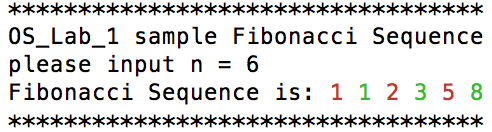
\includegraphics[width=0.5\textwidth]{sample.png}
\end{figure}


\subsection{代码阅读}
~~~~~~仔细阅读《Orange's》的第一章和第二章,深入理解boot.asm文件中的代码,尤其注意问题清单中的问题。

对于下面两行代码:

	 \textbf{mov ax, BootMessage}
	
	\textbf{mov bp, ax}
		
	思考为什么mov bp, ax后,int 10h就能够取到BootMessage了?运行到这行代码的时候
	$ax$里面的值是多少?这个值是不是BootMessage所在内存中的位置(即相对地址还是绝对地址)?
	\begin{itemize}
		\item 这道题目通过阅读Orange‘s或者其他资料即可得到答案,检查时只要说出正确答案就可以通过。如果你只是完成了这项要求,请\underline{\youyuan{提交一个pdf文档}},文档中字数\textbf{少于50字}。
		\item 鼓励同学们进行实验验证,请思考自己认为正确地结论,并通过实验手段进行验证,如果你的验证是可行的、有效的、或者至少是能体现思考的,你将获得一定的\textbf{加分}。完成这项要求的同学,\underline{\youyuan{提交上一项的文档以及实验截图}}。助教检查时,请主动出示截图,并讲解你的实验思路和结果,随机选择同学现场演示其实验过程。
	\end{itemize}


\section{问题清单}
~~~~~~在整个实验的过程中,无论是编程还是查资料,请各位同学注意思考以下问题,助教检查时会从中随机抽取数个题目进行提问,根据现场作答给出分数。
\underline{请注意,我们鼓励自己思考和动手实验},如果
能够提供自己的思考结果并辅助以相应的实验结果进行说明,在分数评定上会酌情考虑。

\begin{enumerate}
	\item boot.asm文件中,\textbf{org~~0700h}的作用
	\item 为什么要把boot.bin放在第一个扇区?直接复制为什么不行?
	\item loader的作用有哪些?
	\item L1,L6各标识了一个字节(8bit)的数据,eax是一个16位寄存器,说明下面每行代码的意思。

\begin{table}
\centering
\begin{tabular}{cc}
行号 & 代码 \\\hline
1 & mov al, [L1] \\
2 & mov eax, L1 \\
3 & mov [l1], ah \\
4 & mov eax, [L6] \\
5 & add eax, [L6] \\
6 & add [L6], eax \\
7 & mov al, [L6]
\end{tabular}
\end{table}
		
	\item \textbf{times 510-(\$-\$\$) db 0}
		
		为什么是510? \$和\$\$分别表示什么?不用times指令怎么写(等价命令)?
		
	\item 解释db命令:\underline{\textbf{L10 db “w”, “o”, “r”, “d”, 0  }}这条语句的意义,并且说明数字0的作用。
	\item \textbf{L1 db 0}
		
		\textbf{L2 dw 1000}
		
		L1、L2是连续存储的吗?即是否L2就存储在L1之后?		
	\item 要是不知道L6标识的是多大的数据,下面这句话对不对?
		
		\textbf{mov [L6], 1}
	\item 如何处理输入输出?在代码中哪里体现出来?
	\item 通过什么来保存前一次的运算结果?在代码中哪里体现出来?
	\item 随机选择代码段,说明作用。
	\item 有哪些段寄存器?
	\item 8086/8088存储单元的物理地址长,CPU总线的数量,可以直接寻址的物理地址空间。
	\item 如何根据逻辑地址计算物理地址?
	\item 寄存器的寻址方式(知道如何计算)。
	\item 几个常用指令的作用(如MOV,LEA等)。
	\item 主程序与子程序的几种参数传递方式。
	
\end{enumerate}

\section{参考资料}
	\begin{enumerate}
		\item 《Orange'S:一个操作系统的实现》
		\item \href{http://www.nasm.us/doc/} {NASM doc}
		\item \href{http://jingliu.me/my_files/nasm.pdf}{Introduction to NASM}
		\item \href{http://www.psut.edu.jo/sites/qaralleh/uplab/doc/MASM_Tutorial.pdf}{MASM Tutorial}
	\end{enumerate}


%\begin{thebibliography}{9}
%\bibitem{nano3}
%  K. Grove-Rasmussen og Jesper Nygård,
%  \emph{Kvantefænomener i Nanosystemer}.
%  Niels Bohr Institute \& Nano-Science Center, Københavns Universitet

%\end{thebibliography}
\end{document}
